%% analyse.tex
%% $Id: analyse.tex 61 2012-05-03 13:58:03Z bless $

\chapter{Analyse}
\label{ch:Analyse}
%% ==============================




%% ==============================
\section{Anforderungen}
%% ==============================
\label{ch:Analyse:sec:Anforderungen}

Um einen Graphen, der zur Diskussion steht auf einen Problemkern zu reduzieren können verschiedene Reduktionsregeln verwendet werden. \\
Zunächst werden die Regeln anhand der folgenden Kriterien beurteilt:
\begin{itemize}
	\item Laufzeit
	\item Erwartete Reduktion
	\item Ressourcenverbrauch
	%\item Wie gut ist das Ergebnis im Vergleich zu anderen Algorithmen?	
\end{itemize}
Dann wird die Anwendung und der Effekt der Regeln auf das eigens erstellte Testset untersucht, um folgende Fragen zu beantworten:
\begin{itemize}
\item Wie effektiv sind die Reduktionsregeln in der Anwendung?
	\begin{itemize}
		\item Wie oft sind die Regeln anwendbar?
		\item Wie viel wird reduziert?
	\end{itemize}
\item Wie (gut) funktionieren die Reduktionsregeln in Kombination?
\item Wie sehen Graphen aus, auf die keine Regel anwendbar ist?
\item Wie sehen Graphen aus, auf die genau eine Regel anwendbar ist?
\end{itemize}

%% ==============================
\section{Bewertung der Reduktionsregeln}
%% ==============================
\label{ch:Analyse:sec:Berwertung}

Um die verwendeten Reduktionsregeln zu bewerten, beziehungsweise zu vergleichen, betrachten wir auf der einen Seite die theoretisch mögliche Reduktion und auf der anderen, wie sich der implementierte Algortihmus verhält. 

%\begin{figure}[htb]
%\centering
 % 	{
\includegraphics[width=.3\textwidth]{Logo-Uni-Trier.jpg}}
%	\caption{Logo der Universität Trier.\label{fig:grafik1}}
%\centering
%\end{figure}


\begin{table}[htb]
\caption{Bewertung der Reduktionsregeln\label{tab:liste}}
\vspace*{1em}
\centering

\bgroup
\def\arraystretch{1.3}%  1 is the default, change whatever you need

\begin{threeparttable}

\begin{tabular}[c]{l|l|c}
	
	\multicolumn{1}{c|}{\textbf{Reduktionsregel}} & 
	\multicolumn{1}{c|}{\textbf{Laufzeit}} & 
	\multicolumn{1}{c}{\textbf{Reduktion}} \\ 
	
	\hline

	Nemhauser-Trotter&$O(k^{3})$&  $\leq 2k$\\
	Kronenregel&$O(\sqrt{|V|}|E|)$ & $\leq 3k$\\
	Buss&$O(k|V|)$  & $\leq k^{2}$\\
	Grad 0&$O(|V|)$& \tnote{*} \\
	Grad 1&$O(|V|)$& \tnote{*} \\
	%Grad 2&$O(n|V|)\ mit\ n\leq1$&\\
	
\end{tabular}

\begin{tablenotes}\footnotesize
\item[*] Die Reduktion dieser Regeln hängt stark von der Struktur des Graphen ab. Eine formale Bestimmung der zu erwartenden Reduktion steht noch aus.
\item \emph{k} beschreibt jeweils den Eingabeparameter der Knotenüberdeckung für einen Graphen $G=(V,E)$
\end{tablenotes}

\end{threeparttable}

\egroup

\end{table}

In Tabelle \ref{tab:liste} stehen die Laufzeiten in der $O$-Notation und erwartete Größe der reduzierten Problemkerns der Nemhauser-Trotter-Regel \cite[S67]{fixed}, der Kronenregel \cite[S71]{fixed} \cite{manual}, die der Buss Regel \cite[S67]{fixed} und von einfachen Reduktionsregeln (Grad 0 und Grad 1) gegenüber. Die Laufzeiten der einfachen Reduktionsregeln ergeben sich folgt:
\begin{proof}
 $Sei\ Graph\ G = (V,E)$
	\begin{align*}
  		Grad\ 0-Reduktion\\
  		\underline{1.Fall:}\ |E|=0&\\
  		&jeder\ Knoten\ aus\ V\ muss\ betrachtet\ werden.\\
  		&\Rightarrow\ Laufzeit:\ O(|V|)\\  		
  		\underline{2.Fall:}\ |E|>0&\\
  		&Sobald\ bei\ der\ Iteration\ ein\ Knoten\ mit\ Grad(v)>0\ (v\in V)\ \\
  		&ausgew\ddot{a}hlt\ wird,\ k\ddot{o}nnen\ alle\ Nachbarn\ ignoriert\ werden.\\
  		&\Rightarrow\ Laufzeit:\ O(x|V|)\ mit\ (x<1)\\
	\end{align*}
\end{proof}
\begin{proof}
$Sei\ Graph\ G = (V,E)$
	\begin{align*}
  		Grad\ 1-Reduktion\\
  		&Sobald\ bei\ der\ Iteration\ ein\ Knoten\ mit\ Grad(v)=1\ (v\in V)\ \\
  		&ausgew\ddot{a}hlt\ wird,\ wird\ der\ Nachbar\ in\ die\ Knotenüberdeckung\\
  		&aufgenommen.\\
  		&\Rightarrow\ Laufzeit:\ O(x|V|)\ mit\ (x<1)\\
	\end{align*}
\end{proof}

TODO was bringt die Bewertung?

%% ==============================
\section{Anwendung der Reduktionsregeln}
%% ==============================
\label{ch:Analyse:sec:Anwendung}
%% ==============================

Das Testset an dem die Algorithmen angewandt wurden besteht aus ungerichteten Graphen, die jeweils eine Knotenmenge von 1000 Knoten und eine Kantenanzahl von 1000 bis 10000 (aufsteigend in 200er Schritten) umfassen. Von jeder \emph{Graphklasse}, die sich durch die Kantenmenge auszeichnet gibt es 20 Exemplare. Dadurch entsteht ein Testset von 900 Graphen. Zum Erstellen der Graphen wurde die LEDA-Funktion \lstinline{random_simple_undirected_graph(|V|,|E|)} \cite{manual} verwendet. Da Zufallsgraphen verwendet werden, gibt es keine Vorgabe für den Parameter \emph{k}. Die obere Beschränkung der Kantenmenge (10000) hat sich bei den Tests ergeben, da ab einer bestimmten Dichte, beziehungsweise Knotenanzahl keine Reduktionsregel mehr erfolgreich ist, beziehungsweise keine Änderung am eingegebenen Graphen mehr erzielte. Dies kann mit der erwarteten Reduktion (siehe Tabelle \ref{tab:liste}) erklärt werden: Je dichter der Graph wird, desto größer wird \emph{k} und sobald $k>\frac{|V|}{2}$ wird, ist bei der Nemhauser-Trotter-Regel und somit auch bei den anderen die theoretische Größe des reduzierten Problemkerns größer oder gleich der Menge der Knoten, was bedeutet, dass theoretisch keine Reduktion stattfinden kann. Daher eignen sich viele Benchmarktests \footnote{http://dimacs.rutgers.edu/pub/challenge/graph/benchmarks/} \footnote{http://sites.nlsde.buaa.edu.cn/~kexu/benchmarks/graph-benchmarks.htm} nicht, da sich diese durch sehr schwere Probleme mit dichten Graphen und Werten für \emph{k}, die sich der Größe der Knotenmenge im jeweiligen Problem annähern, auszeichnen. Eine Knotenmenge von 1000 Knoten pro Graph für das Testset erwies sich bei der Anwendung als ausreichend hoher Wert, um das Einsetzen der Reduktionsregeln zu beobachten.\\
Die Reduktionsregeln wurden jeweils solange auf einen Graphen angewandt, bis sich keine Änderungen mehr ergeben haben. Erzielte mindestens eine der Regeln eine Reduktion, wurde der gesamte Vorgang wiederholt. In der Anwendung sorgte dies dafür, dass für manche Regeln einige weitere Iterationen mögich wurden. In Tabelle \ref{tab:crownSpecial} kann man diesen Effekt beobachten. Die Anwendung der Grad$_{1}$-Regel nach der Kronenregel sorgte dafür, dass bei Graph$_{1}$ 3 und bei Graph$_{2}$ sogar 5 weitere Iterationen der Kronenregel eine Reduktion erzielten.
 Ausgeführt wurden die Experimente auf einem 2.6 GHz, Zweikern, Intel Core i5-3320M mit 8 GB Arbeitsspeicher. In der Tabelle \ref{tab:anwendung} werden die durchschnittliche Anzahl der Anwendungen pro Graph, die durschnittliche Reduktion (Anzahl der Knoten, die aus dem Graphen entfernt wurden), und die durchschnittliche CPU-Zeit, die pro Graph aufgebracht wurde. Die Buss Regel wurde von der Untersuchung ausgeschlossen, da kein Wert für \emph{k} vorliegt, welcher für deren Anwendung essentiell ist, während die restlichen Regeln auch ohne diesen Parameter verwendbar sind.\\
Tabelle \ref{tab:anwendung} spiegelt die erwarteten Werte (\ref{tab:liste}) in soweit wieder, als das die Nemhauser-Trotter-Regel eine deutlich bessere Reduktion als die Kronenregel erreicht, zumindest, wenn sie isoliert angewandt wird. Dabei werden weniger Durchläufe, allerdings ein höherer Rechenaufwand benötigt.

\begin{table}[htb]
\caption{Anwendung einzelner Reduktionsregeln\label{tab:anwendung}}
\vspace*{1em}
\centering

\bgroup
\def\arraystretch{1.3}%  1 is the default, change whatever you need

\begin{threeparttable}

\begin{tabular}[c]{l|l|l|l}
	
	\multicolumn{1}{c|}{\textbf{Reduktionsregel}} & 
	\multicolumn{1}{c|}{\textbf{Anwendungen}} & 
	\multicolumn{1}{c|}{\textbf{Reduktion}} & 
	\multicolumn{1}{c}{\textbf{CPU-Zeit }} \\ 
	
	\hline

	Nemhauser-Trotter& 0.27 &  50.3 & 0.014s\\
	Kronenregel& 0.46 & 19.77 & 0.005s\\
	Grad 1&1.32 & 99.06 & 0.001s\\
	%Grad 2&$O(n|V|)\ mit\ n\leq1$&\\
	
\end{tabular}

\begin{tablenotes}\footnotesize
\item EINFÜGEN
\end{tablenotes}

\end{threeparttable}

\egroup

\end{table}
Während sich die Reduktion durch die Nemhauser-Trotter und die Grad 1 Regel bei der Anwendung an dichteren Graphen, also Graphen mit einer höheren Kantenzahl, erwartungsgemäß stetig verringerte, zeigten sich bei der Kronenregel einige Ausnahmen. Wie in Abbildung \ref{fig:crown} zu sehen ist, setzten sich diese deutlich vom Durchschnitt ab. In Tabelle \ref{tab:crownSpecial} werden die drei Graphen mit einer Kantenmenge über (beziehungsweise gleich) 3000 und einer durch die Kronenregel erreichten Reduktion > 480 Knoten betrachtet. Keiner dieser Graphen ist bipartit.
Bei allen drei Graphen führte die Anwendung der Nemhauser-Trotter-Regel zu keinerlei nennenswertem Effekt, weder isoliert, noch in Kombination mit den anderen Regeln. Ähnlich verhielt sich zunächst die Grad$_{1}$-Regel, wohingegen die Anwendung in Kombination einen großen Einfluss auf die Reduktion hatte. Kombiniert man die Regeln, scheint die Reihenfolge, in der sie eingesetzt werden schwer ins Gewicht zu fallen. Besonders fiel das bei Graph$_{1}$ (3200 Kanten) auf. Wurde zuerst die Grad$_{1}$ und dann die Kronenregel verwendet, war jeweils lediglich ein Durchlauf (Anwendung) zu beobachten. Die Grad$_{1}$-Regel scheint den Graphen derart zu verändern, dass die Stuktur keine Reduktion durch die Kronenregeln mehr zulässt. Betrachtet man dagegen das Ergebnis von Graph$_{2}$, erzeugte die Anwendung in gerade dieser Reihenfolge eine Lösung des Problems: 1000 von 1000 Konten reduziert, wovon 619 eine Knotenüberdeckung für Graph$_{2}$ bilden. Auch hier war die Reihenfolge wieder wichtig, wie man bei der Reduktionsmenge beim entgegengesetzten Experiment (erst Kronenregel, dann Grad$_{1}$-Regel) sieht, wo 858 Knoten bei der Reduktion aus dem Graphen entfernt wurden. Bei Graph$_{1}$ und Graph$_{3}$ zeichnet sich der übrig gebliebene Problemkern nach der jeweils größten Reduktion dadurch aus, dass der Großteil der Knoten vom Grad 2 ist. Der Problemkern $G'_{3}$ von Graph$_{3}$, zu sehen in  Abbildung \ref{fig:crownRest}, lässt sich in die Knotenmengen $V_{1}$ und $V_{2}$  mit $|V_{1}| = |V_{2}| = 5$ aufteilen. Bis auf die Knoten $v_{1} \in V_{1}$ und $v_{2} \in V_{2}$, welche vom Grad 3 sind, hat jeder andere Knoten in  $G'_{3}$ durch die vorherige Reduktion den Grad 2. Für  $v_{1}$ und $v_{2}$ existiert eine Kante $(v_{1}, v_{2})$ in $G'_{3}$, welche die Knotenmengen verbindet. Innerhalb der Knotenmengen existiert einen Zyklus (Kreis), mit ungerader Knotenzahl, woraus sich folgern lässt, dass $G'_{3}$ nicht bipartit ist. Hier ist keine der Reduktionsregeln mehr erfolgreich.
\begin{figure}[htb]
\centering
  	{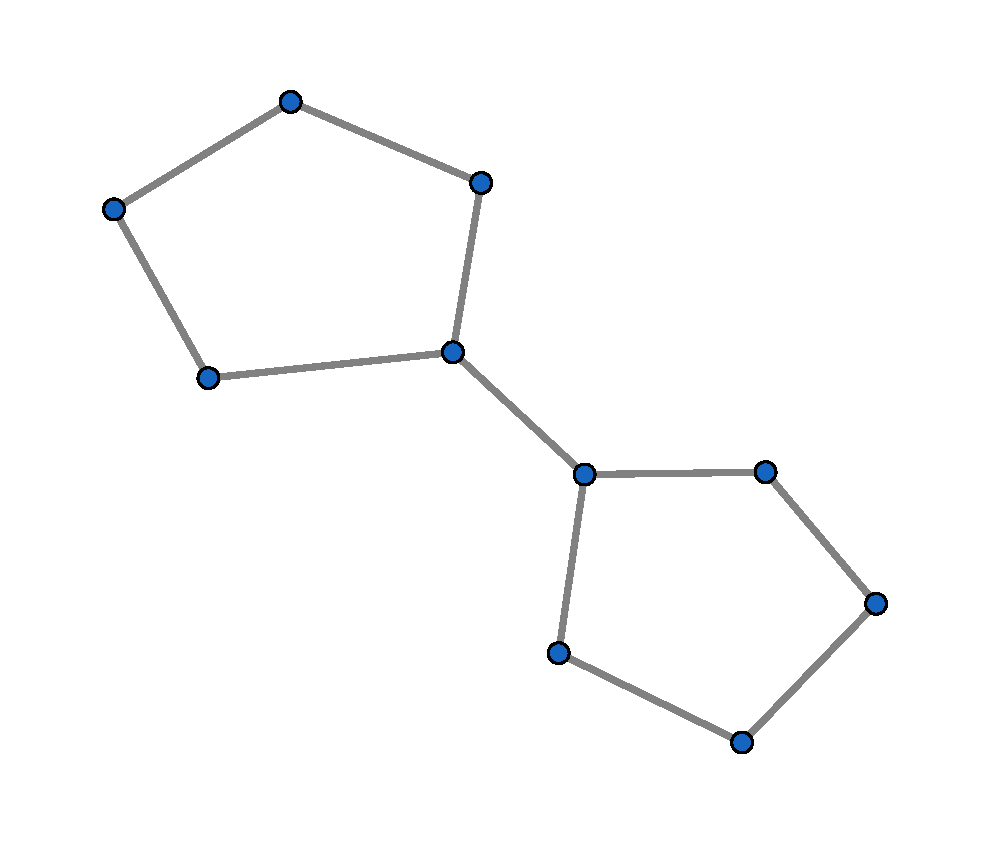
\includegraphics[width=0.3\textwidth]{crownRest.pdf}}
	\caption{Graph$_{3}$ nach Anwendung von Grad$_{1}$-Regel und Kronenregel.\label{fig:crownRest}}
\centering
\end{figure}
\begin{figure}[htb]
\centering
  	{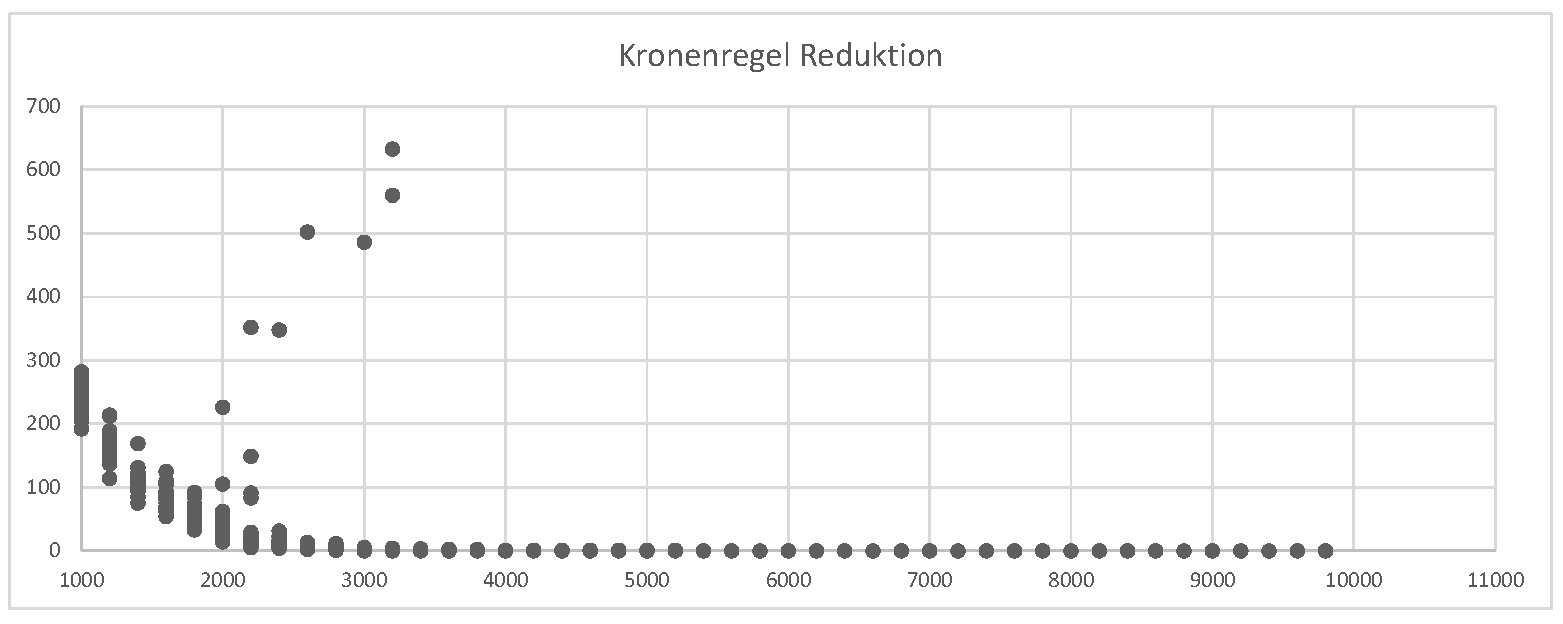
\includegraphics[width=\textwidth]{analysisCrown.pdf}}
	\caption{Anwendung der Kronenregel.\label{fig:crown}}
\centering
\end{figure}

\begin{table}[htb]
\caption{Besondere Graphen für die Kronenregel \label{tab:crownSpecial}}
\vspace*{1em}
\centering

\bgroup
\def\arraystretch{1.3}%  1 is the default, change whatever you need

\begin{threeparttable}

\begin{tabular}[c]{l|l|l|l|l}
	
	\multicolumn{1}{c|}{\textbf{Graph}} & 
	\multicolumn{1}{c|}{\textbf{Reduktionsregeln}} & 
	\multicolumn{1}{c|}{\textbf{Anwendungen$_{1}$}} &
	\multicolumn{1}{c|}{\textbf{Anwendungen$_{2}$}} &
	\multicolumn{1}{c}{\textbf{Reduktion}} \\ 
	
	\hline
		
	Graph$_{1}$ & Kronenregel& 11 & - & 560\\
	& Nemhauser-Trotter & 1 & - & 4\\
	& Grad$_{1}$ & 1 & - & 18 \\
	& Grad$_{1}$-Kronenregel & 1 & 1 & 22\\
	& Kronenregel - Grad$_{1}$ & 14 & 11 & 946\\
	
	\hline

	Graph$_{2}$ & Kronenregel & 13 & - & 486\\
	& Nemhauser-Trotter & 1 & - & 6\\
	& Grad$_{1}$ & 2 & - & 40 \\
	& Grad$_{1}$-Kronenregel & 12 & 13 & 1000\\
	& Kronenregel - Grad$_{1}$ & 18 & 12 & 858\\

	\hline	
	
	Graph$_{3}$ & Kronenregel & 15 & - &633\\	
	& Nemhauser-Trotter & 1 & - & 4\\
	& Grad$_{1}$ & 2 & - & 46 \\
	& Grad$_{1}$-Kronenregel & 18 & 11 & 990\\
	& Kronenregel - Grad$_{1}$ & 15 & 9 & 971\\
	


	
	
\end{tabular}
\begin{tablenotes}\footnotesize
\item EINFÜGEN
\end{tablenotes}

\end{threeparttable}

\egroup

\end{table}

Die in Tabelle \ref{tab:kombination} zusammengefassten Ergebnisse zeigen, dass die Nemhauser-Trotter-Regel in Kombination mit anderen Regeln nicht die gleiche Reduktion erzeugt, wie Grad$_{1}$ und Kronenregel. Des Weiteren lassen sich eine Reihe von Beobachtungen anstellen.
\begin{figure}[htb]
\centering
  	{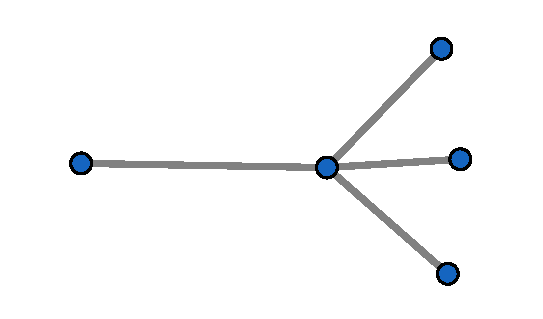
\includegraphics[width=0.3\textwidth]{restkrone.pdf}}
	\caption{Einfache Krone\label{fig:restcrown}}
\centering
\end{figure}
\\
Da durch die Grad$_{1}$-Regel einfache 1-gradige Knoten, beziehungsweise deren Nachbarn und damit der Kopf einer einfachen Krone, reduziert wird, stellt sie eine vereinfachte Form der Kronenregel dar. Daher sollten intuitiv nach der erschöpfenden Anwendung der Kronenregel kaum Probleminstanzen, bei denen die Grad$_{1}$-Regel erfolgreich ist, übrig bleiben. Wie die Tabelle allerdings zeigt, ist die Kombination beider Regeln im Vergleich zu den anderen Zweierkombination diejenige, die am meißten Knoten aus den Problemgraphen entfernt. Zu dem besseren Ergebnis der Reduktion kommmt hier noch die stark erhöhte durchschnittliche Anwendung pro Graph. Ein Grund hierfür könnte die Auswahl des ersten Matchings in der Kronenregel sein, welches maßgeblich für die darauffolgende Reduktion ist. Eine "einfache" Krone, wie sie in Abbildung \ref{fig:crownRest} zu sehen ist, wird mit großer Wahrscheinlichkeit von der Kronenregel, so wie sie hier verwendet wird, ignoriert. Im Abschnitt \ref{ch:Implementierung:sec:Kronenregel} wird genauer erläutert, warum das der Fall ist: Bei der Anwendung auf das Testset wird die größte Reduktion mit der Kronenregel dann erreicht, wenn bei der Erstellung des Matchings $M_{1}$ zunächt Kanten betrachtet werden, bei denen beide Knoten höhergradig, genauer gesagt einen höheren Grad, als der durchschnittliche Knoten im akutellen Graphen haben. Wäre die abgebildete Krone Teil eines größeren Graphen, kann es sein, dass der Kopf dieser Krone nicht in das Matching $M_{1}$ aufgenommen und so bei der weiteren Reduktion nicht berücksichtigt wird. Die Grad$_{1}$-Regel reduziert demnach jene einfachen Kronen, die von der Kronenregel ignoriert, beziehungsweise nicht erkannt werden. Ändert man nun die Reihenfolge, in der die beiden Regeln angewandt werden, zeigen sich nur minimale Änderungen in der durchschnittlichen Reduktion und der durchschnittlichen Anwendung pro Graph. Das könnte die Vermutung stützen, dass die Grad$_{1}$-Regel und die Kronenregel überwiegend verschiedene Arten von Kronen abdecken, da annähernd gleiche Ergebnisse unabhängig von der Reihenfolge der Regeln erzielt werden. Die Unterschiede in den Ergebnissen zeichnen sich dadurch aus, dass die als Zweites verwendete Regel im Schnitt weniger Anwendungen hat, als wenn sie als Erstes verwendet wird. Für die Kronenregel bedeutet das eine Differenz von 0.42 durchschnittlichen Durchläufen, für die Grad$_{1}$-Regel nur 0.07. Diese 0.07 Grad$_{1}$-Regel-Durchläufe mehr pro Graph verschlechtern allerdings die Gesamtreduktion. Diesen Effekt kann auch bei dem Extrembespiel von Graph${_1}$ in Tabelle \ref{tab:crownSpecial} beobachten, wo der gleiche Effekt eintritt. Es scheint also im Großteil der Fälle für eine maximale Reduktion von Vorteil zu sein, wenn die Kronenregel vor der Grad$_{1}$-Regel angewandt wird, was die die anderen Beispielen in Tabelle \ref{tab:kombination} wiederum untermalen.\\ \\
Betrachtet man die Grad$_{1}$-Regel in Kombination mit der Nemhauser-Trotter-Regel sorgt die Reihenfolge zwar für einen Unterschied in der durchschnittlichen Anwendung, allerdings ist das Ergebnis der Reduktion identisch. Ein Teil der von der Grad$_{1}$-Regel abgedeckten Reduktion wird auch von der Nemhauser-Trotter-Regel entfernt und dem entsprechend auch anders herum. Die Differenz bei verschiedener Reihenfolge beträgt bei der Grad$_{1}$-Regel 0.2 und bei der NT-Regel 0.26 Iterationen pro Graph, was vermuten lässt, dass die Grad$_{1}$-Regel Bereiche des Graphen, wo beide Regeln greifen effizienter, mit weniger Durchläufen entfernt. Vergleicht man diese Kombination mit einer Grad$_{1}$-Kronenregel-Reduktion, fällt auch auf, dass die Form des Graphen, die die Nemhauser-Trotter-Regel durch das Entfernen von Knoten und Kanten erzeugt, die Anwendungsmöglichkeit der Grad$_{1}$-Regel einschränkt. In die andere Richtung scheint diese Einschränkung auch zu gelten. Die gesamte Reduktion pro Graph erhöht sich nicht sonderlich, vergleicht man die Werte, die die Grad$_{1}$-Regel alleine erzeugt (Tabelle \ref{tab:anwendung}). \\ \\
Kronenregel und Nemhauser-Trotter-Regel sorgen in Kombination dafür, dass die jeweilige Anwendung pro Graph leicht erhöht wird. Auch zeigt sich ein deutlicher Anstieg der Reduktion pro Graph im Vergleich zur Einzelanwendung, was darauf hindeutet, dass die beiden Regeln wiederum verschiedene Bereiche des Graphen entfernen. Bei den Dreierkombinationen zeigt sich dieser Trend ebenfalls: Wird hier die Kronenregel unmittelbar vor der Nemhauser-Trotter-Regel angewandt, finden deutlich mehr Iterationen (der NT-Regel) pro Graph statt, als es bei vorheriger Verwendung der Grad$_{1}$-Regel der Fall ist. Zwei Interessante Ergebnisse liefern die Kombinationen Grad$_{1}$ - Nemhauser-Trotter - Kronenregel und Grad$_{1}$ - Kronenregel - Nemhauser-Trotter. Die Position, beziehungsweise die Reihenfolge der Regeln beeinflusst die Anwendungshäufigkeit von Grad$_{1}$ und Nemhauser-Trotter-Regel deutlich, während Gesamtreduktion und Anwendungen der Kronenregel annähernd gleich bleiben. Dies könnte wiederum ein Indikator dafür sein, dass NT und Grad$_{1}$-Regel ähnliche Teile des Graphen reduzieren und die Kronenregel den Graphen scheinbar für die jeweilige Reduktion günstig verändert.
Werden Nemhauser-Trotter-Regel, Kronenregel und Grad$_{1}$-Regel in dieser Reihenfolge angewandt, kann im Schnitt die größte Reduktion pro Graph erreicht werden. In Abbildung \ref{fig:trottCrownOne} lassen sich wiederum einige Ausnahmen erkennen: Zwei Graphen stechen besonders aus dem Durchschnitt heraus, zu sehen in Tabelle \ref{tab:trottCrownOneSpecial}. Zum Einen ein Graph mit 2000 Kanten und einer Reduktion von lediglich 195 Knoten (Graph$_{4}$), während andere Graphen dieser Größe annähernd komplett gelöst wurden. Zum Anderen ein Graph mit 7200 Kanten, bei dem 762 Knoten entfernt werden konnten (Graph$_{5}$). Keiner der Graphen ist - weder vor noch nach der Reduktion - regulär oder bipartit. Die Kronenregel greift bei Graph$_{5}$ nur, wenn die Grad$_{1}$-Regel den einen eingradigen und dessen Nachbarknoten entfernt. Bis auf die Grad$_{1}$-Regel kann keine Reduktionsregel auch nur einen Knoten des Graphen entfernen, wenn sie alleine angewandt werden. Eine weitere interessante Beobachtung für Graph$_{5}$ ist, dass die Konfiguration für die Kronenregel sehr wichtig für eine hohe Reduktion ist. Die Knoten des Graphen haben vor der Reduktion einen durchschnittlichen Grad von 14 (abgerundet). Werden beim finden des Matchings $M_{1}$ zunächst Kanten, bei denen jeder Knoten den Grad $\geq$ 14 hat bevorzugt, kann findet keine Reduktion statt, auch nicht in Kombination mit den anderen Regeln. Wählt man als Einschränkung stattdessen Grad > 14 werden 702 Knoten reduziert. Das Beste Ergebnis wird bei einer Konfiguration erreicht, bei der der Grad beider Knoten größer, als der durchschnittliche Grad aller Knoten ist. Auf dieses Phänomen wird in Kapitel \ref{ch:Implementierung:sec:Kronenregel} weiter eingegangen. Bei Graph$_{4}$ zeigt sich, wie bei Graph$_{5}$, dass die Nemhauser-Trotter-Regel keinen Einfluss auf die Gesamtreduktion hat. Kronenregel und Grad$_{1}$-Regel entfernen in Kombination die Größte Menge an Knoten.


\begin{figure}[htb]
\centering
  	{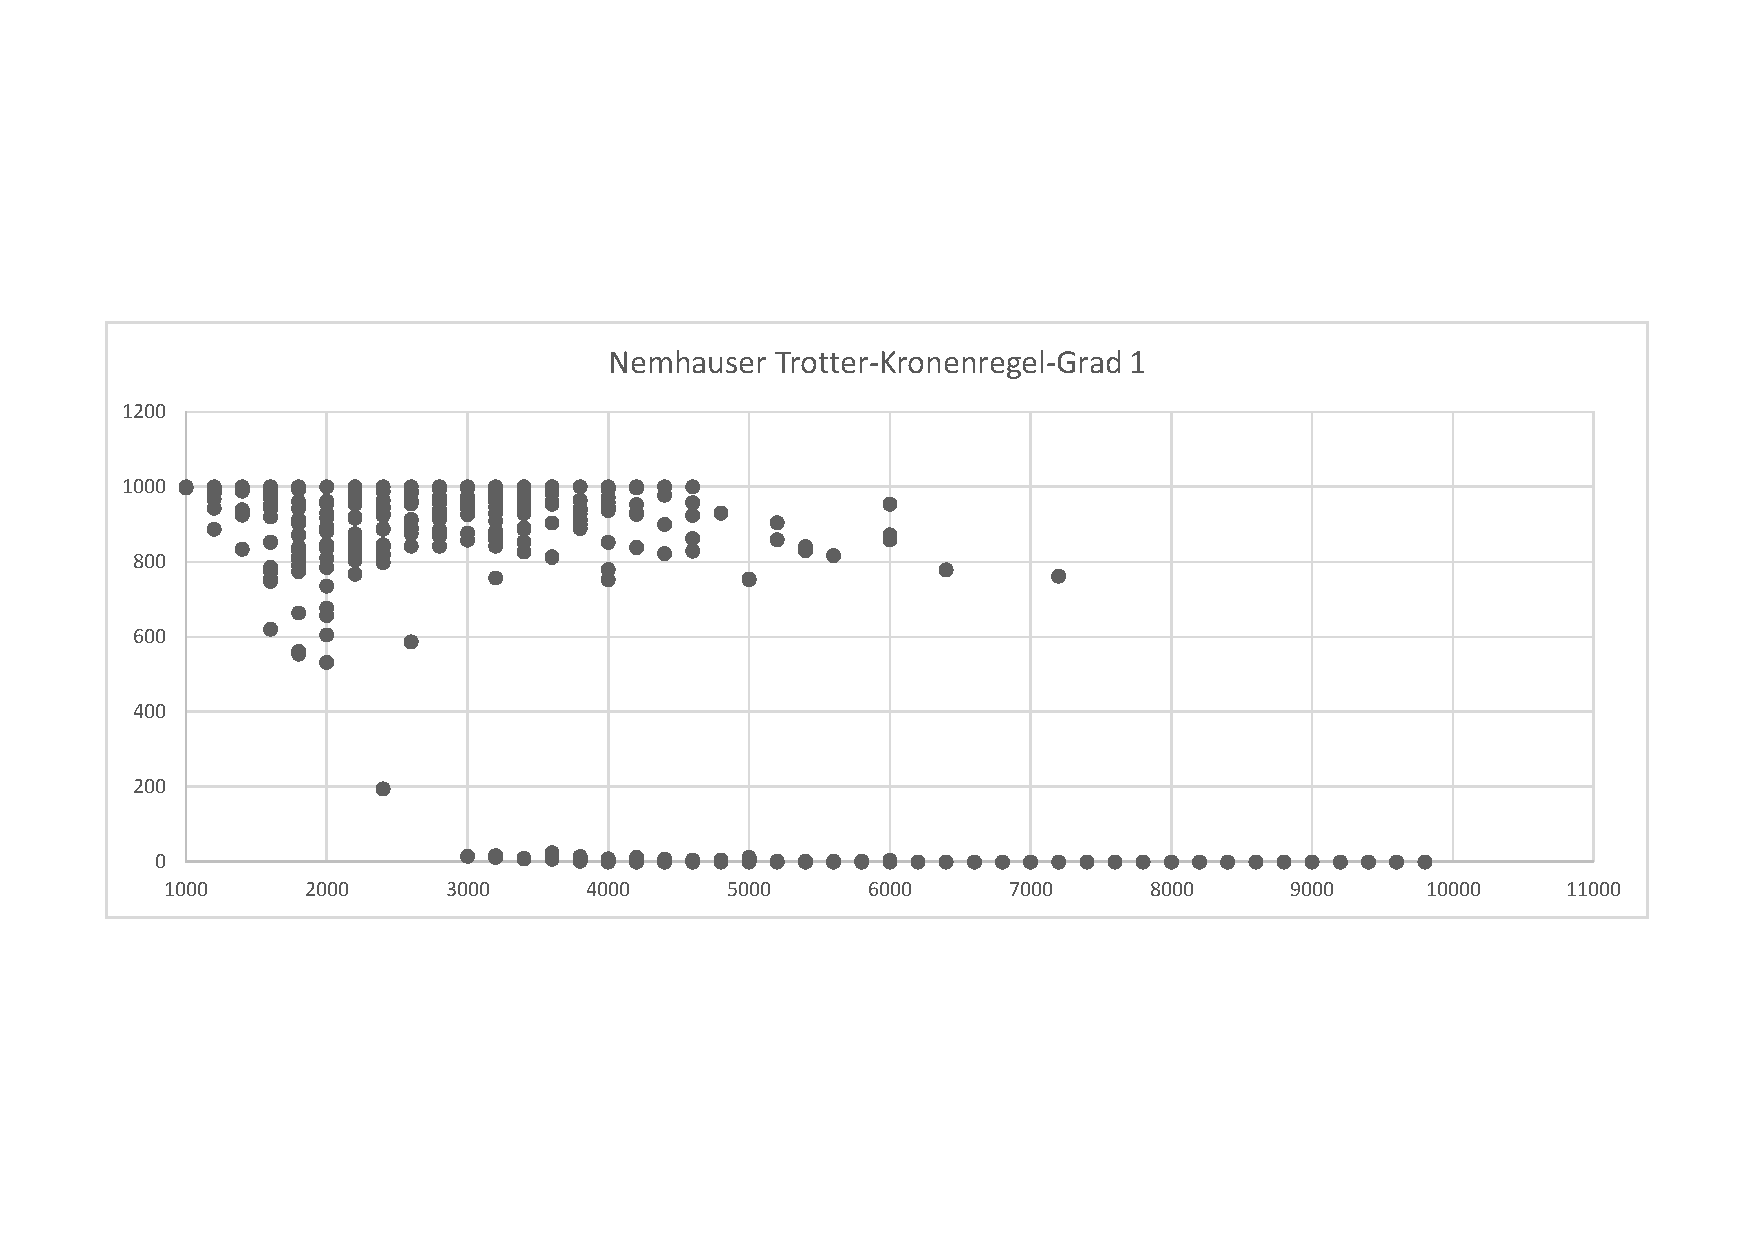
\includegraphics[width=\textwidth]{analysisTrott_Crown_One.pdf}}
	\caption{Anwendung von Nemhauser-Trotter-Regel, Kronenregel und Grad$_{1}$-Regel.\label{fig:trottCrownOne}}
\centering
\end{figure}


\begin{table}[htbp]
\caption{Anwendung kombinierter Reduktionsregeln\label{tab:kombination}}
\vspace*{1em}
\centering

\bgroup
\def\arraystretch{1.3}%  1 is the default, change whatever you need

\begin{threeparttable}

\begin{tabular}[c]{l|l|l|l|l}
	
	\multicolumn{1}{c|}{\textbf{Kombination}} &
	\multicolumn{1}{c|}{\textbf{Anwendungen$_{1}$}} &
	\multicolumn{1}{c|}{\textbf{Anwendungen$_{2}$}} &
	\multicolumn{1}{c|}{\textbf{Anwendungen$_{3}$}} & 
	\multicolumn{1}{c}{\textbf{Reduktion}} \\
	\hline

	K - G$_{1}$ & 3.63 & 4.3 & - &331.8\\
	G$_{1}$ - K & 4.37 & 3.22 & - &331.17\\
	K - NT & 0.8 & 0.38 & - & 68.28 \\
	NT - K & 0.45 & 0.56 & - & 68.6\\
	G$_{1}$ - NT & 1.33 & 0.017 & - & 99.87\\
	NT - G$_{1}$ & 0.28 & 1.13 & - & 99.87\\
	K  - G$_{1}$ - NT & 3.61 & 4.29 & 0.11 & 334.67 \\
	K - NT - G$_{1}$ & 3.6 & 0.87 & 3.39 & 334.83 \\
	G$_{1}$ - NT - K & 4.36 & 0.12 & 3.2 & 334.17 \\
	G$_{1}$ - K - NT & 3.61 & 3.2 & 0.65 & 334.16 \\
	NT - K - G$_{1}$ & 0.39 & 3.44 & 4.03 & 335.2 \\
	NT - G$_{1}$ - K & 0.91 & 3.42 & 3.2 & 334.16 \\

	
\end{tabular}

\begin{tablenotes}\footnotesize
\item EINFÜGEN
\end{tablenotes}

\end{threeparttable}

\egroup

\end{table}


\begin{table}[htb]
\caption{Besondere Graphen für die Dreierkombinationen von Regeln\label{tab:trottCrownOneSpecial}}
\vspace*{1em}
\centering

\bgroup
\def\arraystretch{1.3}%  1 is the default, change whatever you need

\begin{threeparttable}

\begin{tabular}[c]{l|l|l|l|l|l}
	
	\multicolumn{1}{c|}{\textbf{Graph}} & 
	\multicolumn{1}{c|}{\textbf{Reduktionsregeln}} & 
	\multicolumn{1}{c|}{\textbf{Anwend.$_{1}$}} &
	\multicolumn{1}{c|}{\textbf{Anwend.$_{2}$}} &
	\multicolumn{1}{c|}{\textbf{Anwend.$_{3}$}} &
	\multicolumn{1}{c}{\textbf{Reduktion}} \\ 
	
	\hline
		
	Graph$_{4}$ & NT - K - G$_{1}$ & 1 & 5 & 6 & 195 \\
	& G$_{1}$ - NT - K & 6 & 0 & 5 & 195 \\
	& Nemhauser-Trotter & 1 & - & - & 11 \\
	& Kronenregel & 1 & - & - & 11 \\
	& Grad$_{1}$ & 2 & - & - & 91 \\
	& Kronenregel - Grad$_{1}$ & 6 & 5 & - & 195 \\
	
	\hline

	Graph$_{5}$ & NT - K - G$_{1}$ & 1 & 9 & 2 & 762 \\
	& Nemhauser-Trotter & 0 & - & - & 0\\
	& Kronenregel & 0 & - & - & 0\\
	& Grad$_{1}$ & 1 & - & - & 2 \\
	& Kronenregel - Grad$_{1}$ & 9 & 3 & - & 762\\
	
	
\end{tabular}
\begin{tablenotes}\footnotesize
\item EINFÜGEN
\end{tablenotes}

\end{threeparttable}

\egroup

\end{table}




\begin{table}[htb]
\caption{Statistiken über Graph$_{5}$\label{tab:graph4}}
\vspace*{1em}
\centering

\bgroup
\def\arraystretch{1.3}%  1 is the default, change whatever you need

\begin{threeparttable}

\begin{tabular}[c]{ l | l | l | | l | l}
	
	\multicolumn{1}{c|}{\textbf{Status}} & 
	\multicolumn{1}{c|}{\textbf{Grad der Knoten}} & 
	\multicolumn{1}{c||}{\textbf{Knoten}} &
	\multicolumn{1}{c|}{\textbf{Grad der Knoten}} & 
	\multicolumn{1}{c}{\textbf{Knoten}}\\
	
	\hline
		
	Vor der Reduktion & 0 & 0 &15  & 106 \\
	& 1 & 1 & 16&99 \\
	& 2 & 1 & 17& 84\\
	& 3 & 0 & 18& 66\\
	& 4 & 1 & 19& 39\\
	& 5 & 3 & 20& 27\\
	& 6 & 12 & 21& 16\\
	& 7 & 13 & 22& 18\\
	&  8& 17 & 23& 6\\
	&  9& 37 & 24& 3\\
	&  10& 65 & 25& 4\\
	&  11& 59 & 26& 5\\
	&  12& 101 & 27& 3\\
	&  13& 99 & 28& 1\\
	&  14& 114 & & \\
	
	\hline

	Nach der Reduktion & 0 & 0 & 6 & 18 \\
	& 1 & 0 & 7 & 11 \\
	& 2 & 55 & 8 & 8 \\
	& 3 & 59 & 9 & 0 \\
	& 4 & 46 & 10 & 0 \\
	& 5 & 41 & 11 & 1 \\
	
	
\end{tabular}
\begin{tablenotes}\footnotesize
\item EINFÜGEN
\end{tablenotes}

\end{threeparttable}

\egroup

\end{table}

%% ==============================
\section{Interpretation der Ergebnisse}
%% ==============================
\label{ch:Analyse:sec:Interpretation}
%% ==============================

\begin{itemize}
\item Gegenüberstellung der Reduktionsergebnisse
\item Graphen werden dichter $\Rightarrow$ \emph{k} erhöht sich $\Rightarrow$ Keine Reduktion mehr erfolgreich
\item 
\end{itemize}


\section{Zusammenfassung}
%% ==============================
\label{ch:Analyse:sec:zusammenfassung}

Am Ende sollten ggf. die wichtigsten Ergebnisse nochmal in \emph{einem}
kurzen Absatz zusammengefasst werden.

%%% Local Variables: 
%%% mode: latex
%%% TeX-master: "thesis"
%%% End: 
